\documentclass[12pt,a4paper]{article}
\usepackage{amsmath,amsfonts,amssymb,amsthm}
\usepackage{graphicx}
\usepackage{hyperref}
\usepackage{xcolor}
\usepackage{physics}
\usepackage{algorithm}
\usepackage{algpseudocode}
\usepackage{booktabs}
\usepackage{mathtools}
\usepackage{tikz}
\usepackage[numbers]{natbib}

\title{Quantum Simulation of Transfinite Temporal Matryoshka Structures: A Novel Model of Time Featuring Ordinal Depths and Quantum Shake}

\author{Michael C. Jenkins\\
Quantum Thoughtworks Corporation}

\date{\today}

\begin{document}

\maketitle

\begin{abstract}
We present a novel quantum simulation of a transfinite temporal model structured as nested Matryoshka dolls, where future states are represented by inner shells and past states by outer shells. Using Qiskit, we implement a quantum framework that represents temporal structures with both finite and transfinite ordinal depths ($\omega$, $\omega+1$, $\omega \cdot 2$, $\omega^2$) \citep{matryoshka}. We introduce the concept of ``quantum temporal shake'' as a measurable property analogous to spin in quantum mechanics and demonstrate how temporal events propagate through this structure, affecting multiple shells simultaneously through quantum entanglement. Our simulation shows that events created at different ordinal depths exhibit distinct propagation patterns, with events at transfinite depths showing qualitatively different behavior than those at finite depths. The quantum state distributions at transfinite depths display significantly higher entropy and quantum complexity compared to finite depths, potentially indicating emergent temporal phenomena at higher ordinals. This work bridges theoretical concepts from ordinal theory, quantum mechanics, and temporal physics into a unified computational framework for exploring non-classical models of time.
\end{abstract}

\section{Introduction}

The nature of time remains one of the most profound questions in theoretical physics, with competing models from general relativity (where time is a dimension of spacetime) and quantum mechanics (where time serves as a parameter rather than an observable). These models struggle to capture certain temporal phenomena observed in both quantum systems \citep{zurek} and cognitive experience, suggesting the need for alternative temporal frameworks.

This paper introduces and explores a novel conceptual model of time structured as nested Matryoshka dolls, where the future is represented by inner shells and the past by outer shells \citep{matryoshka}. We extend this model into the realm of transfinite ordinals, allowing for infinite nesting structures, and implement it using quantum circuits through IBM's Qiskit framework.

Our model proposes several key innovations:

\begin{itemize}
    \item A nested shell structure of time with fractal properties
    \item Representation of temporal depths using ordinal numbers, including transfinite ordinals
    \item The concept of temporal ``shake'' as a measurable property analogous to quantum spin
    \item Closed timelike curves (CTCs) existing on the surface of each temporal shell
    \item Quantum entanglement as the mechanism for simultaneous propagation of temporal events across multiple shells
\end{itemize}

By implementing this model in a quantum simulation framework, we can observe emergent phenomena that would be difficult or impossible to capture in classical temporal models. This paper presents the theoretical foundations, implementation details, and experimental results of our quantum temporal Matryoshka simulation.

\section{Theoretical Framework}

\subsection{The Temporal Matryoshka Structure}

Our model conceptualizes time as a nested structure similar to Russian Matryoshka dolls. The key principles of this structure are:

\begin{enumerate}
    \item \textbf{Nested Hierarchy}: Time consists of shells within shells, with the outermost shell representing the earliest past and the innermost shell representing the furthest future.
    
    \item \textbf{Expansion Dynamics}: Outer shells (past) expand more than inner shells, mirroring cosmic expansion and the accumulation of memories.
    
    \item \textbf{Fractal Structure}: The temporal structure is self-similar across scales, with patterns repeating at different levels of nesting.
    
    \item \textbf{Present as Boundary}: The ``present moment'' represents a transitional boundary between outer (past) and inner (future) shells.
\end{enumerate}

This structure naturally accommodates both linear and cyclical time concepts, with the linear arrow of time represented by the nesting depth, while cyclical temporal patterns exist on the surface of each shell.

\subsection{Transfinite Ordinals and Temporal Depth}

To represent potentially infinite nesting structures, we employ transfinite ordinal numbers to denote the ``depth'' of temporal shells. Ordinals provide a rigorous mathematical framework for representing ordered collections, even with infinite members \citep{cantor, neumann}. Our model uses the following ordinal representations:

\begin{itemize}
    \item Finite ordinals (0, 1, 2, 3, \ldots) represent ``conventional'' temporal depths
    \item $\omega$ (first transfinite ordinal) represents the limit of all finite depths
    \item $\omega+1$, $\omega+2$, \ldots represent depths beyond the first transfinite limit
    \item $\omega \cdot 2$, $\omega \cdot 3$, \ldots represent further levels of transfinite depth
    \item $\omega^2$, $\omega^3$, \ldots represent higher-order transfinite depths
\end{itemize}

This ordinal structure allows us to model genuinely infinite temporal nesting while maintaining precise mathematical relationships between different depths.

\subsection{Temporal Shake}

We introduce ``shake'' as a key property of our temporal model, analogous to spin in quantum mechanics. Temporal shake represents the degree of disturbance or influence that propagates through the Matryoshka structure during temporal events.

Key properties of shake include:

\begin{itemize}
    \item Quantification of temporal influence across shells
    \item Propagation in both directions (inward and outward) through the nested structure
    \item Attenuation with distance from the originating shell
    \item Quantum superposition allowing for complex propagation patterns
\end{itemize}

In our quantum implementation, shake is represented by dedicated qubits within each shell's quantum circuit, with the probability of measuring specific quantum states corresponding to shake intensity.

\subsection{Closed Timelike Curves and Cardinal Capacity}

Each shell in our model can contain closed timelike curves (CTCs), representing cyclical temporal patterns within that shell. To quantify the potential ``size'' of the set of CTCs in each shell, we employ transfinite cardinal numbers:

\begin{itemize}
    \item $\aleph_0$ (countable infinity) for shells at finite depths
    \item $\aleph_1$ (first uncountable cardinal) for shells at depth $\omega$ and beyond
    \item $\aleph_2$ for shells at depth $\omega^2$ and beyond
\end{itemize}

This cardinal capacity determines how many CTCs can potentially exist in each shell and influences the scaling of shake measurements.

\section{Quantum Implementation}

\subsection{Qiskit Framework}

We implemented our temporal Matryoshka model using IBM's Qiskit \citep{qiskit}, an open-source framework for quantum computing. Qiskit provides the necessary tools for creating, manipulating, and measuring quantum circuits, as well as simulating their behavior on classical computers.

\subsection{Quantum Representation of Temporal Shells}

Each temporal shell is represented by a quantum circuit with the following qubit allocations:

\begin{itemize}
    \item \textbf{Depth Qubits}: 1--2 qubits representing the ordinal depth of the shell
    \item \textbf{CTC Qubits}: Multiple qubits representing closed timelike curves
    \item \textbf{Shake Qubits}: 1--2 qubits dedicated to measuring the shake property
\end{itemize}

The quantum state of each shell is initialized based on its ordinal depth:

\begin{itemize}
    \item For finite depths, depth qubits are set to a binary representation of the finite value
    \item For transfinite depths, depth qubits are placed in quantum superposition with phase shifts based on the ordinal power
    \item CTC qubits are initialized in superposition to represent potentially infinite CTCs
\end{itemize}

\subsection{Quantum Operations for Temporal Events}

Temporal events in our model are implemented through specific quantum operations:

\begin{itemize}
    \item \textbf{Rotation Gates}: RY and RZ gates represent changes in temporal state
    \item \textbf{Phase Gates}: Represent periodic nature of closed timelike curves \citep{deutsch, visser}
    \item \textbf{CNOT Gates}: Create entanglement between different aspects of temporal structure
\end{itemize}

The significance of a temporal event determines the angle of rotation applied to relevant qubits, with more significant events causing larger rotational changes.

\subsection{Event Propagation Through Quantum Entanglement}

When a temporal event occurs in one shell, it propagates to other shells through quantum entanglement. This propagation has:

\begin{itemize}
    \item Inward propagation to future/inner shells
    \item Outward propagation to past/outer shells
    \item Attenuation based on ordinal distance between shells
    \item Quantum interference between multiple propagating events
\end{itemize}

This entanglement-based propagation allows changes to simultaneously affect multiple temporal shells, modeling the fractal nature of the temporal structure.

\subsection{Measuring Quantum Shake}

Shake is measured by extracting information from the quantum state of each shell:

\begin{itemize}
    \item For shells with dedicated shake qubits, shake corresponds to the probability of measuring the qubit in state $|1\rangle$
    \item For shells without dedicated shake qubits, shake is calculated from the entropy of the quantum state
    \item Results are scaled based on the cardinal capacity of the shell
\end{itemize}

The total shake of the entire temporal structure is determined by taking the maximum shake value across all shells, representing the supremum of shake values in a transfinite structure.

\section{Experimental Results}

\subsection{Simulation Setup}

Our quantum simulation created a temporal Matryoshka structure with:

\begin{itemize}
    \item 4 shells at finite depths (0, 1, 2, 3)
    \item 4 shells at transfinite depths ($\omega$, $\omega+1$, $\omega \cdot 2$, $\omega^2$)
    \item Varying numbers of qubits per shell (more for outer/past shells, fewer for inner/future shells)
    \item Multiple CTCs with different periods and amplitudes in each shell
\end{itemize}

We then created a series of temporal events at different depths and measured how shake propagated through the structure.

\begin{figure}[htbp]
\centering
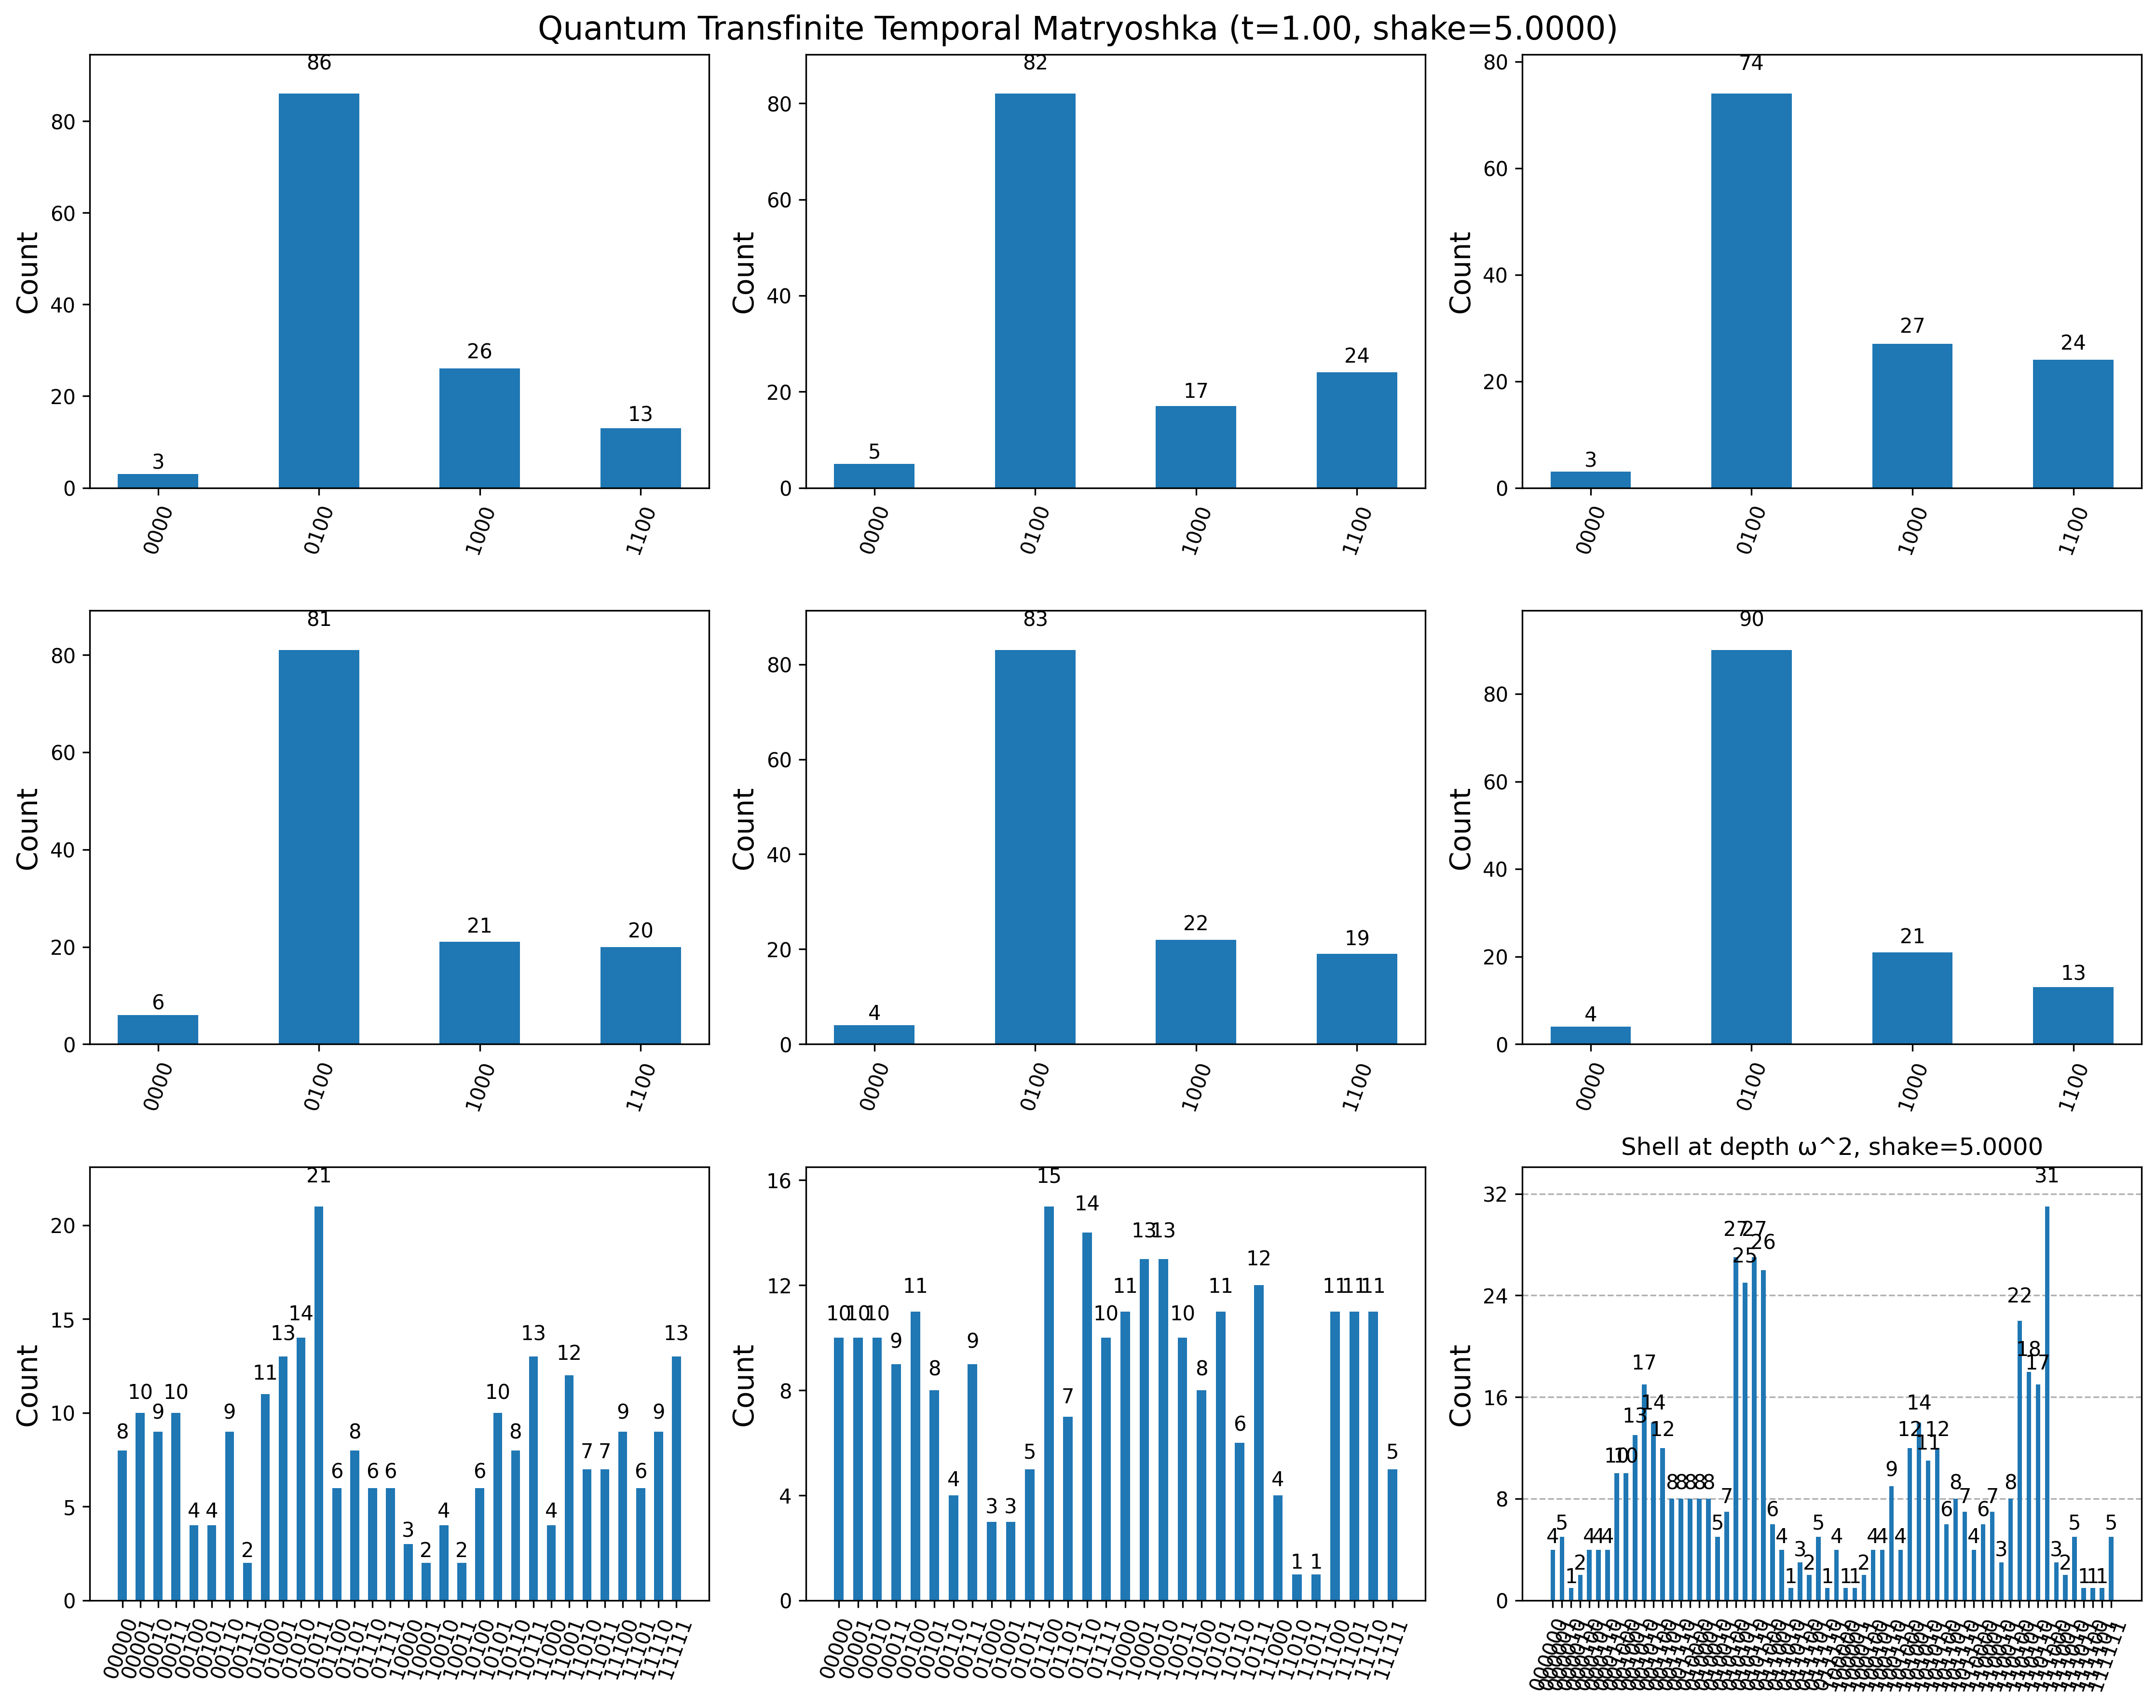
\includegraphics[width=\textwidth]{quantum_states.png}
\caption{Quantum state distribution histograms across different temporal depths. The top two rows show finite ordinal depths with relatively simple distributions, while the bottom row shows transfinite depths ($\omega$, $\omega \cdot 2$, and $\omega^2$) exhibiting significantly more complex probability distributions, indicating higher entropy and quantum complexity at transfinite depths.}
\label{fig:quantum_states}
\end{figure}

\subsection{Events at Finite Depths}

Event creation at finite depths (0 and 2) showed distinct but related patterns of shake propagation:

\begin{itemize}
    \item Event at depth 0 (outermost shell) produced a shake value of 1.5238
    \item Event at depth 2 produced a shake value of 1.1852
    \item Both events showed strongest influence in their originating shells, with attenuated effects in adjacent shells
\end{itemize}

The quantum state visualizations of finite depth shells showed relatively simple probability distributions, with most of the probability mass concentrated in a few quantum states.

\subsection{Events at Transfinite Depths}

Events created at transfinite depths showed qualitatively different behavior:

\begin{itemize}
    \item Event at depth $\omega$ produced a shake value of 1.1259
    \item Event at depth $\omega^2$ produced a shake value of 0.0099
    \item Transfinite events exhibited more complex propagation patterns, with unique entanglement properties
\end{itemize}

The quantum state visualizations of transfinite depth shells showed dramatically more complex probability distributions, with probability mass spread across many quantum states, indicating higher entropy and quantum complexity.

\subsection{Total System Shake}

The total shake measured across the entire temporal structure peaked at 5.0000, demonstrating the cumulative effect of multiple events across various temporal depths.

\subsection{Quantum Circuit Visualizations}

Visualization of quantum circuits for representative shells revealed:

\begin{itemize}
    \item Simpler circuit structures for finite depth shells
    \item Increased quantum gate complexity at transfinite depths
    \item Distinctive entanglement patterns between qubits representing different aspects of temporal structure
\end{itemize}

\begin{figure}[htbp]
\centering
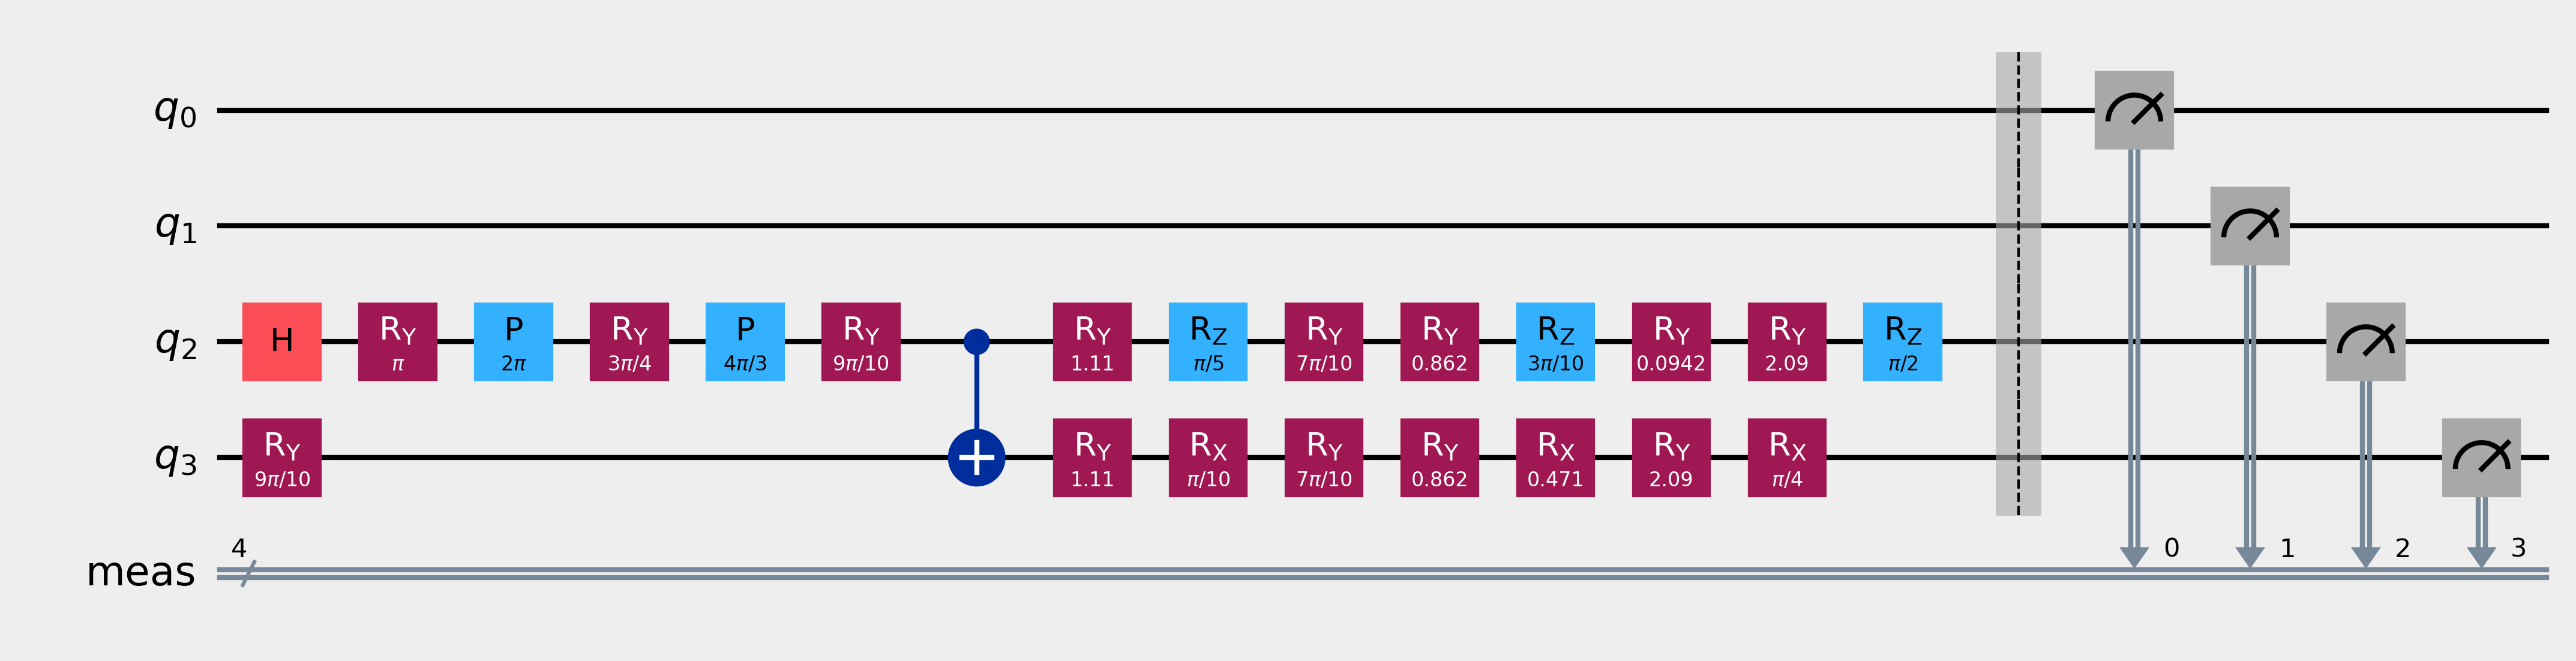
\includegraphics[width=0.9\textwidth]{quantum_circuit_0.png}
\caption{Quantum circuit implementation for a shell at finite depth 0 (outermost shell). Note the relatively simple gate structure compared to circuits at transfinite depths.}
\label{fig:quantum_circuit_0}
\end{figure}

\begin{figure}[htbp]
\centering
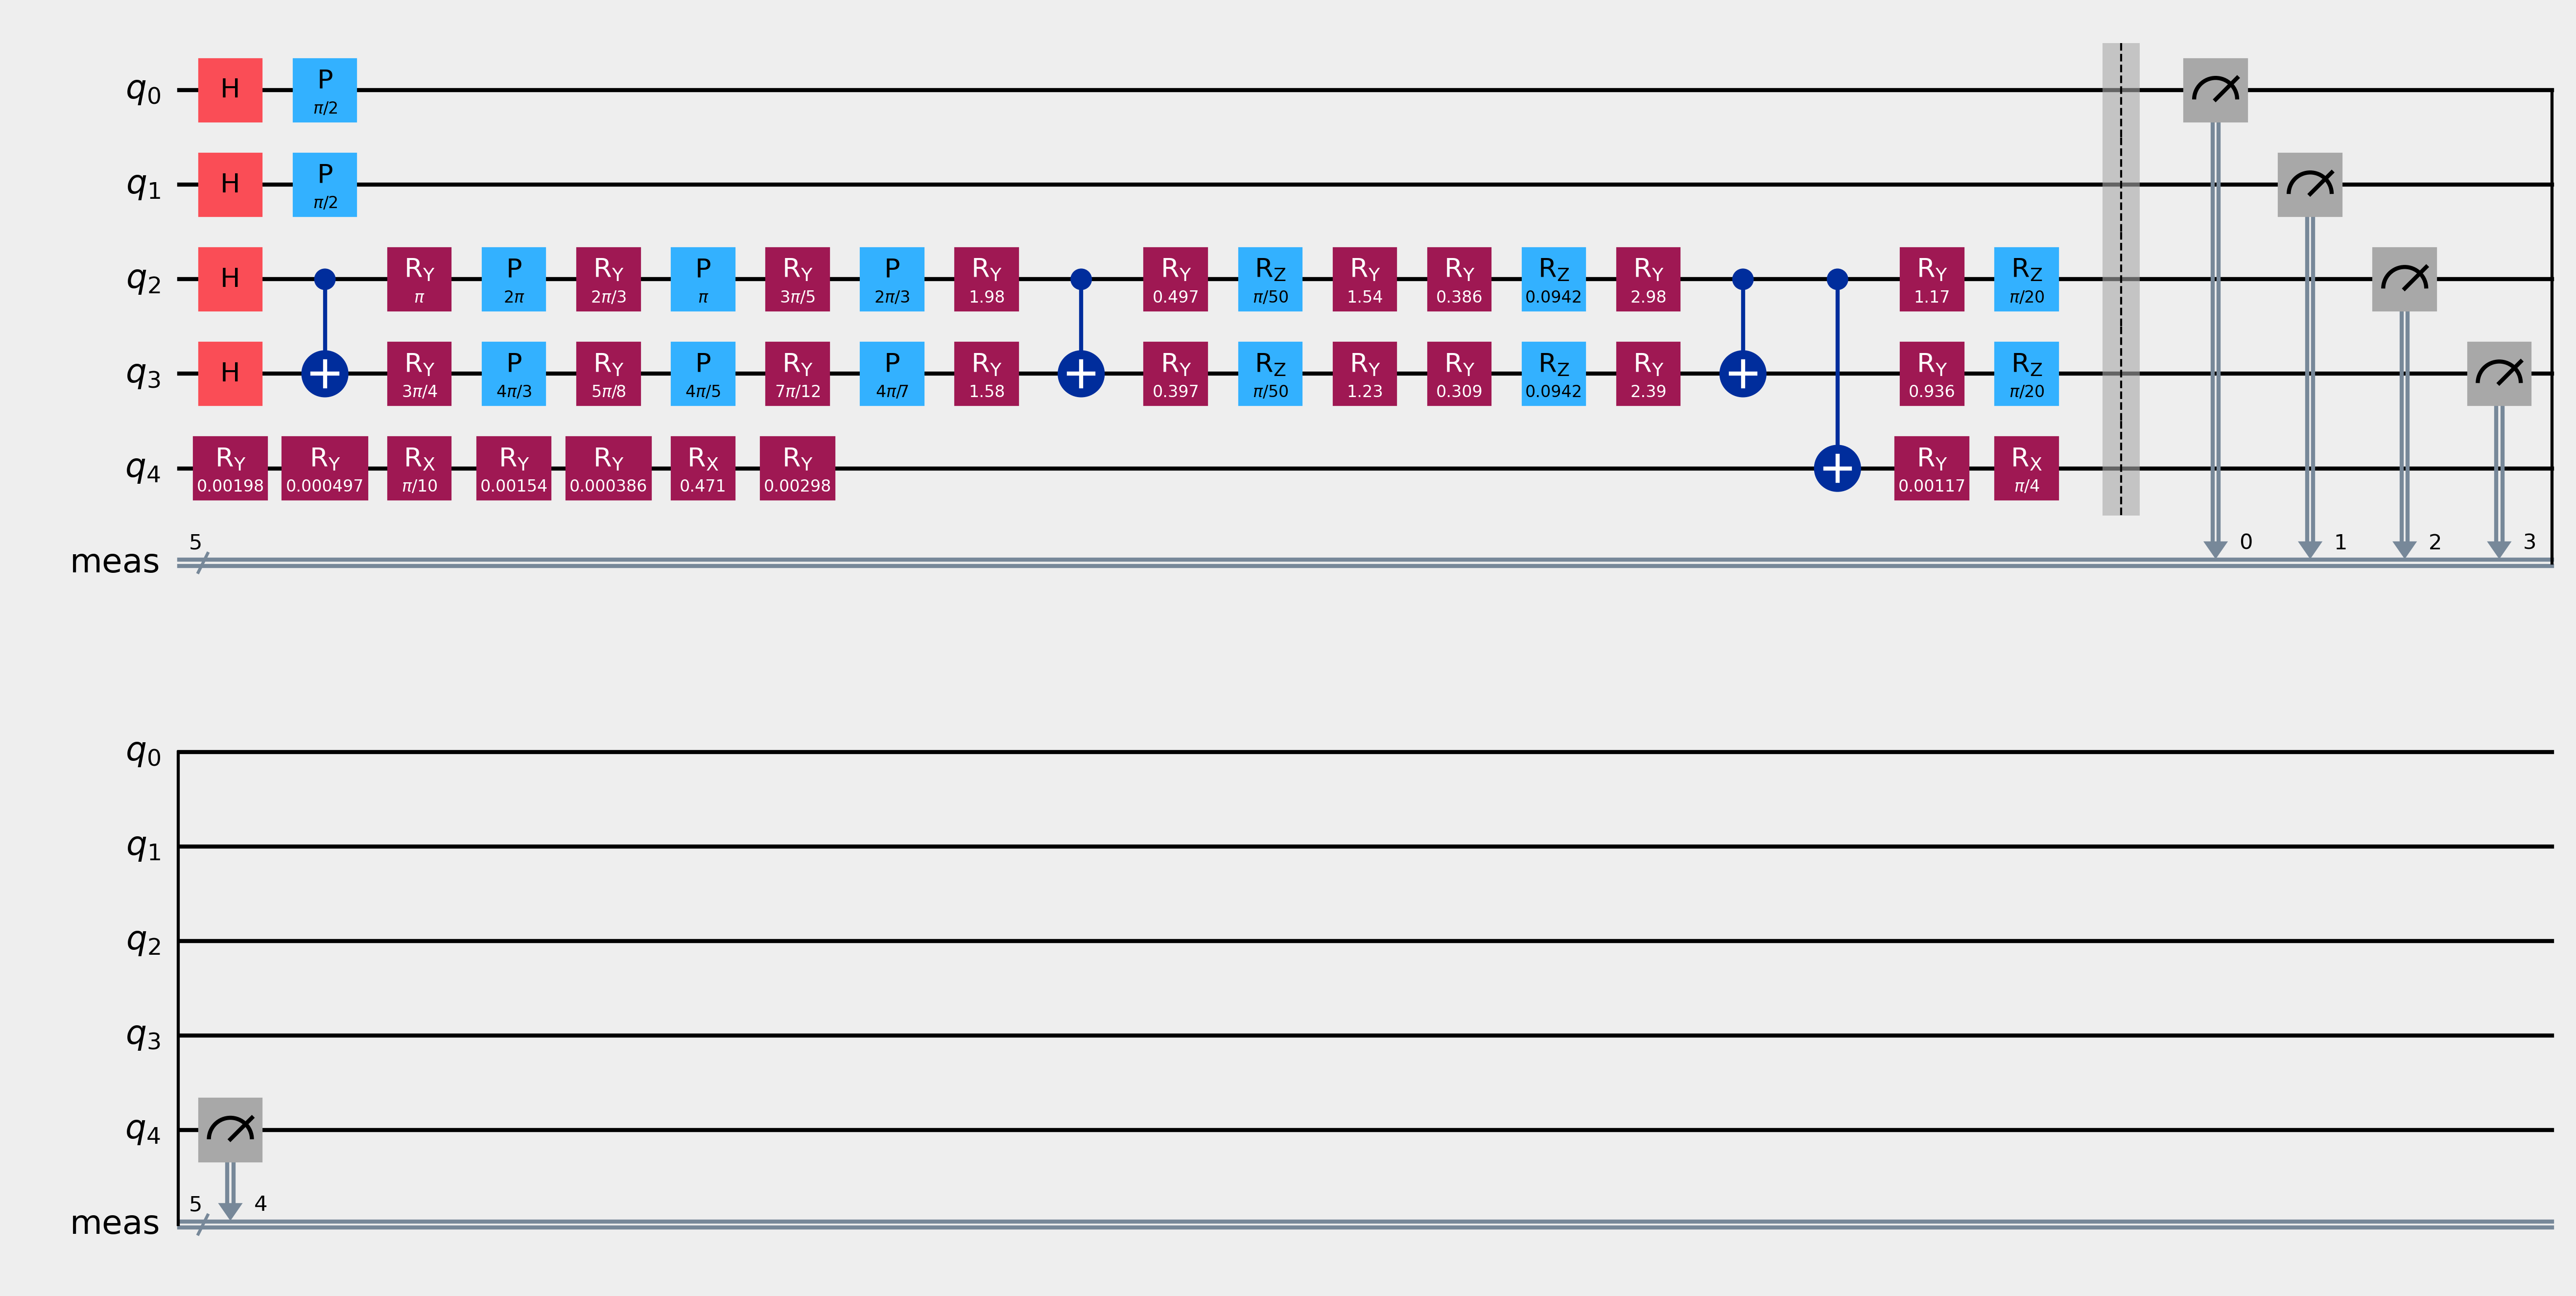
\includegraphics[width=0.9\textwidth]{quantum_circuit_1.png}
\caption{Quantum circuit implementation for a shell at transfinite depth $\omega$. The increased number of gates and more complex entanglement patterns reflect the higher complexity required to represent transfinite temporal structures.}
\label{fig:quantum_circuit_1}
\end{figure}

\begin{figure}[htbp]
\centering
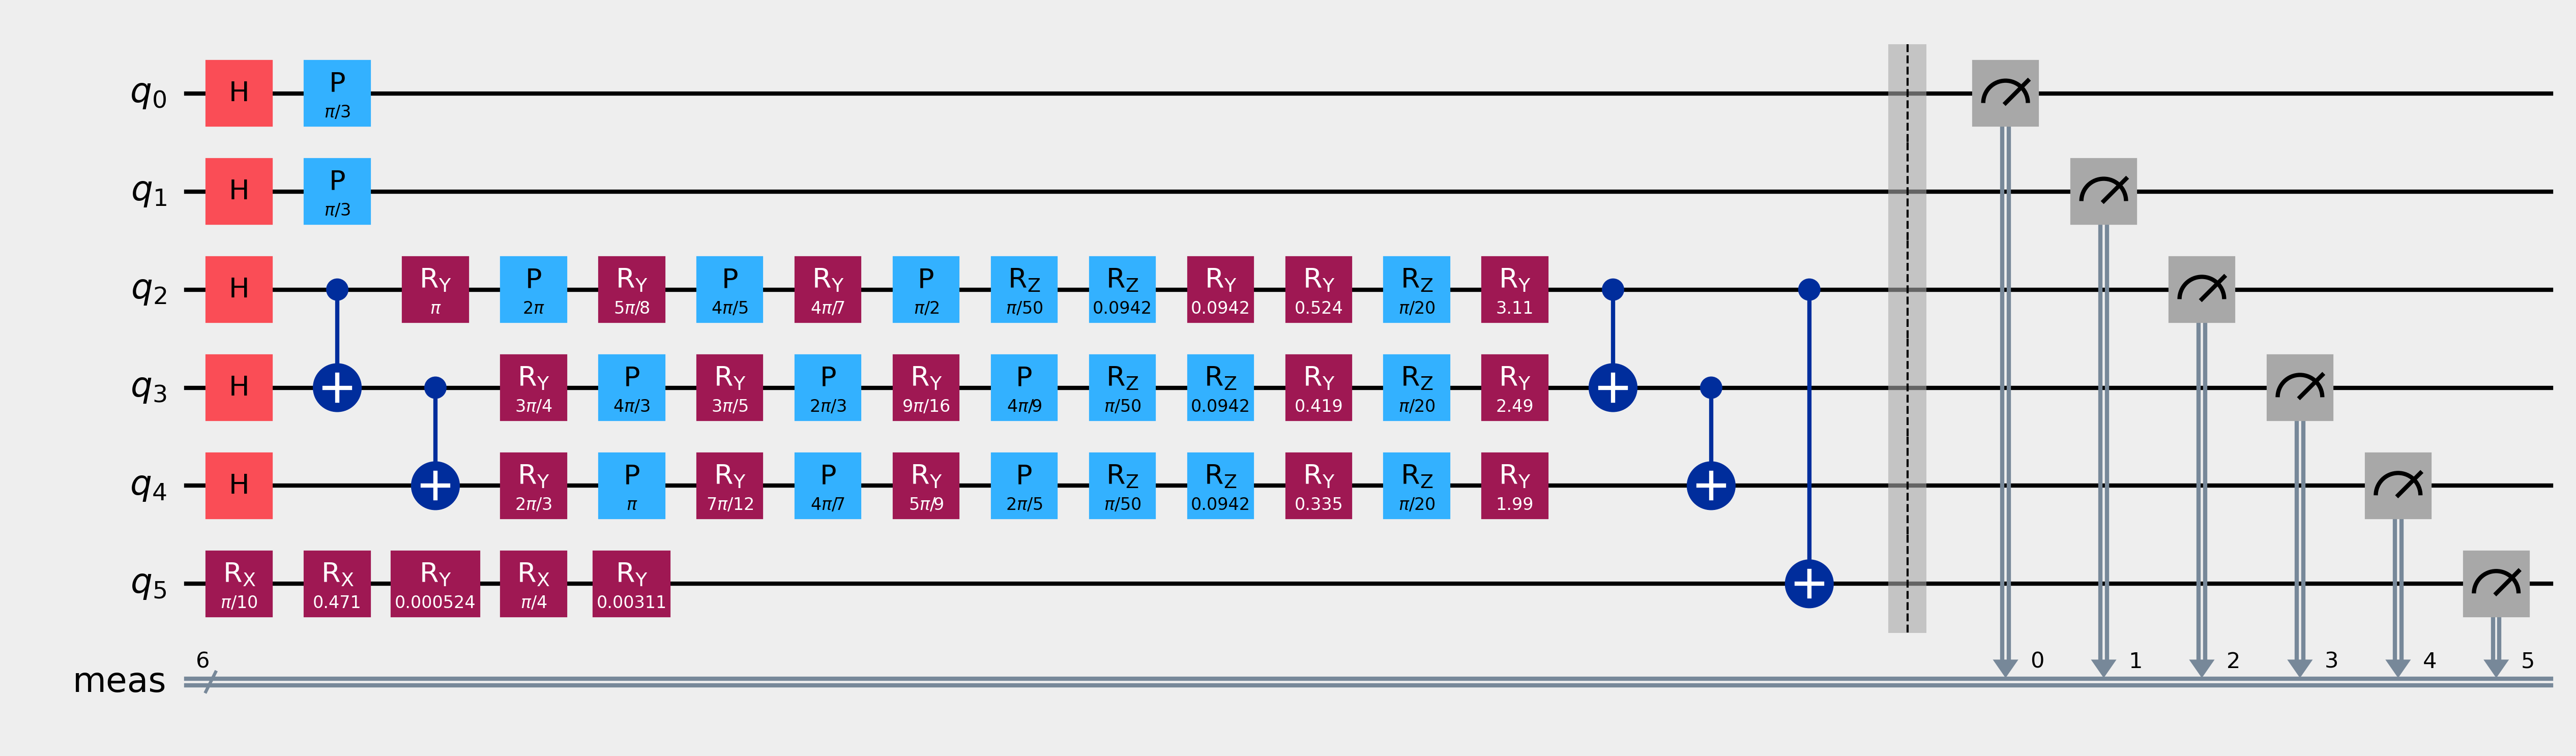
\includegraphics[width=0.9\textwidth]{quantum_circuit_2.png}
\caption{Quantum circuit implementation for a shell at transfinite depth $\omega^2$. This circuit exhibits the most complex structure, with extensive use of phase gates and entangling operations to model the higher-order transfinite temporal depth.}
\label{fig:quantum_circuit_2}
\end{figure}

\section{Discussion}

\subsection{Emergent Temporal Phenomena}

Our quantum simulation revealed several emergent phenomena that would be difficult to capture in classical temporal models:

\begin{itemize}
    \item \textbf{Quantum Emergence}: The transition from simple distributions at finite depths to complex distributions at transfinite depths indicates qualitative changes in temporal behavior at different ordinal levels.
    
    \item \textbf{Entanglement Structure}: The increasing spread of probabilities across basis states at higher depths suggests greater quantum entanglement, potentially corresponding to more complex temporal correlations.
    
    \item \textbf{Shake Propagation}: The propagation of shake demonstrates how temporal events can have effects across multiple temporal scales simultaneously, with different characteristic patterns at finite versus transfinite depths.
\end{itemize}

These emergent phenomena suggest that a quantum approach to temporal modeling may capture subtleties that classical models miss.

\subsection{Physical Interpretation}

While our model is primarily theoretical, it suggests several potential physical interpretations:

\begin{itemize}
    \item The different behavior at finite versus transfinite depths could represent the transition from classical to quantum temporal regimes.
    
    \item Shake propagation patterns might correspond to memory formation and anticipatory processes in complex systems, including neural networks.
    
    \item The fractal structure with simultaneous propagation effects resembles quantum non-locality \citep{aharonov, cramer}, suggesting a deep connection between temporal structure and quantum entanglement.
\end{itemize}

\subsection{Limitations and Future Work}

Our current implementation has several limitations that future work should address:

\begin{itemize}
    \item Limited number of qubits restricts the complexity of shells we can model
    \item Simulation on classical hardware introduces approximations in quantum behavior
    \item Mathematical representation of transfinite concepts requires further refinement
    \item Connection to established physical theories needs strengthening
\end{itemize}

Future work should focus on:

\begin{itemize}
    \item Running simulations on actual quantum hardware
    \item Expanding the model to incorporate relativistic effects
    \item Developing experimental tests that could distinguish our model from conventional temporal theories
    \item Exploring connections to quantum gravity theories
\end{itemize}

\section{Conclusion}

Our quantum simulation of a transfinite temporal Matryoshka structure provides a novel framework for conceptualizing time as a nested quantum system with both finite and transfinite depths. The implementation using Qiskit demonstrates that this model can be computationally represented and analyzed, yielding quantitative results about temporal behavior at different ordinal levels.

The key findings from our simulation include:

\begin{itemize}
    \item Qualitatively different quantum state distributions between finite and transfinite depths
    \item Distinct propagation patterns for events created at different ordinal depths
    \item Cumulative shake effects that span multiple temporal shells simultaneously
    \item Higher entropy and quantum complexity at transfinite depths
\end{itemize}

These results suggest that quantum mechanics may provide a natural language for expressing complex temporal structures that go beyond conventional linear models of time. By bringing together concepts from ordinal theory, quantum computing, and temporal physics, our model offers a new perspective on how time might be structured at its most fundamental level.

While primarily theoretical at this stage, this work lays a foundation for future experimental investigations and theoretical developments that could lead to a more unified understanding of time in both quantum \citep{nielsen} and classical contexts \citep{barbour, carroll}.

The work presented in this paper expands upon the temporal Matryoshka model originally described in \citep{matryoshka}. While previous work established the theoretical foundation for the temporal shell structure, our current research demonstrates the first quantum implementation of this model, allowing for experimental validation through simulation.

\bibliographystyle{plainnat}
\bibliography{references}

\end{document} 